\documentclass[10pt,a4paper]{article}

% --- Core Packages & Times New Roman Typography ---
\usepackage[utf8]{inputenc}
\usepackage[T1]{fontenc}
\usepackage{newtxtext,newtxmath} % Times New Roman for text and math
\usepackage[margin=0.8in, headheight=14pt]{geometry}
\usepackage{amsmath}
\usepackage{booktabs}
\usepackage{tabularx}
\usepackage{listings}
\usepackage{xcolor}
\usepackage{microtype}
\usepackage{enumitem}
\usepackage{titlesec}
\usepackage{fancyhdr}
\usepackage{lastpage}
\usepackage[most]{tcolorbox}
\usepackage{graphicx}
\usepackage{hyperref}
\graphicspath{{./}}

% --- Google Research / Technical Design Color Palette ---
\definecolor{gblue}{HTML}{1A73E8}
\definecolor{gdark}{HTML}{202124}
\definecolor{gslate}{HTML}{5F6368}
\definecolor{gbg}{HTML}{F8F9FA}
\definecolor{gborder}{HTML}{DADCE0}
\definecolor{gred}{HTML}{D93025}
\definecolor{ggreen}{HTML}{188038}

\hypersetup{
    colorlinks=true,
    linkcolor=gblue,
    citecolor=gblue,
    urlcolor=gblue,
    pdftitle={Idempotent Webhook Ingestion Engine with Crash-Safe Local Durability},
    pdfauthor={Candidate Assessment Report}
}

% --- Section Heading Styling ---
\titleformat{\section}
  {\normalfont\large\bfseries\color{gdark}}{\thesection}{0.6em}{}[\vspace{-0.3em}\textcolor{gborder}{\titlerule[0.5pt]}]
\titleformat{\subsection}
  {\normalfont\normalsize\bfseries\color{gdark}}{\thesubsection}{0.5em}{}
\titlespacing*{\section}{0pt}{1.3ex plus 0.3ex minus .2ex}{0.8ex plus .1ex}
\titlespacing*{\subsection}{0pt}{1.0ex plus 0.2ex minus .1ex}{0.5ex plus .1ex}

% --- Running Headers & Footers ---
\pagestyle{fancy}
\fancyhf{}
\fancyhead[L]{\footnotesize\textcolor{gslate}{\textbf{Technical Design Report} $\cdot$ Idempotent Webhook Inbox}}
% \fancyhead[R]{\footnotesize\textcolor{gslate}{Tenant Isolation $\cdot$ Monotonic Replay $\cdot$ POSIX Durability}}
\fancyfoot[L]{\footnotesize\textcolor{gslate}{Software Engineering Assessment}}
\fancyfoot[R]{\footnotesize\textcolor{gslate}{Page \thepage\ of \pageref*{LastPage}}}
\renewcommand{\headrulewidth}{0.4pt}
\renewcommand{\footrulewidth}{0.4pt}
\renewcommand{\headrule}{\hbox to\headwidth{\color{gborder}\leaders\hrule height \headrulewidth\hfill}}
\renewcommand{\footrule}{\hbox to\headwidth{\color{gborder}\leaders\hrule height \footrulewidth\hfill}}

% --- Code Listings Configuration ---
\lstdefinestyle{codeblock}{
    backgroundcolor=\color{gbg},
    basicstyle=\ttfamily\footnotesize\color{gdark},
    breaklines=true,
    captionpos=b,
    commentstyle=\color{gslate}\itshape,
    frame=single,
    frameround=tttt,
    rulecolor=\color{gborder},
    keywordstyle=\color{gblue}\bfseries,
    stringstyle=\color{gred},
    numbers=left,
    numberstyle=\tiny\color{gslate},
    numbersep=8pt,
    tabsize=4,
    showstringspaces=false,
    xleftmargin=14pt,
    xrightmargin=6pt,
    framesep=5pt,
    aboveskip=6pt,
    belowskip=4pt
}
\lstset{style=codeblock}

% --- Custom Callout Box ---
\newtcolorbox{calloutbox}[1]{
    enhanced,
    colback=gbg,
    colframe=gborder,
    borderline west={2.5pt}{0pt}{gblue},
    coltitle=gdark,
    colbacktitle=gbg,
    fonttitle=\bfseries\small,
    title={#1},
    arc=1pt,
    boxrule=0.5pt,
    left=8pt,
    right=8pt,
    top=4pt,
    bottom=4pt
}

\begin{document}

% --- Google-Style Technical Report Header ---
\vspace*{-1.5em}
\noindent{\color{gblue}\rule{\textwidth}{1.5pt}}
\vspace{0.2em}

\noindent{\LARGE\bfseries\color{gdark} Idempotent, Monotonic Webhook Ingestion Engine with Crash-Safe Local State Durability}

\vspace{0.5em}
\noindent{\normalsize\textbf{Candidate Assessment Report} $\cdot$ Software Engineering Practice} \\
{\footnotesize\color{gslate} October 18, 2026 }
\vspace{0.4em}

\begin{tcolorbox}[colback=gbg, colframe=gborder, boxrule=0.5pt, arc=2pt, left=10pt, right=10pt, top=6pt, bottom=6pt]
\footnotesize\noindent\textbf{\color{gdark}Abstract ---}
At-least-once webhook delivery introduces duplicate packets, out-of-order versions, status collisions, and mid-write crash risks. This paper presents a zero-dependency Python 3.10+ ingestion engine that enforces tenant isolation, deduplicates payloads via canonical matching, guarantees monotonic version progression, and persists state via atomic POSIX \texttt{os.replace}. We formalize six Architectural Decision Records (ADRs)—highlighting immediate key reservation on version conflicts (Row 9 replay hazard) and strict boolean type exclusion—and verify the system across three fixture stages and 18 unit tests with zero byte mutations on corrupt state.
\end{tcolorbox}
\vspace{0.3em}

\section{Problem Formulation}

Upstream webhook publishers use timeout-driven retries with exponential backoff, exposing receivers to four failure modes (Figure~\ref{fig:problem_diagram}):
\begin{enumerate}[leftmargin=1.5em, noitemsep, topsep=2pt]
    \item \textbf{Duplicate Ingestion:} Identical payloads redelivered after network timeouts.
    \item \textbf{Stale Hazards:} Out-of-order older versions arriving after newer state transitions.
    \item \textbf{Version Conflicts:} Contradictory statuses arriving at the same version number.
    \item \textbf{Truncated Writes:} Process termination corrupting in-place file writes.
\end{enumerate}

\begin{figure}[htbp]
\centering
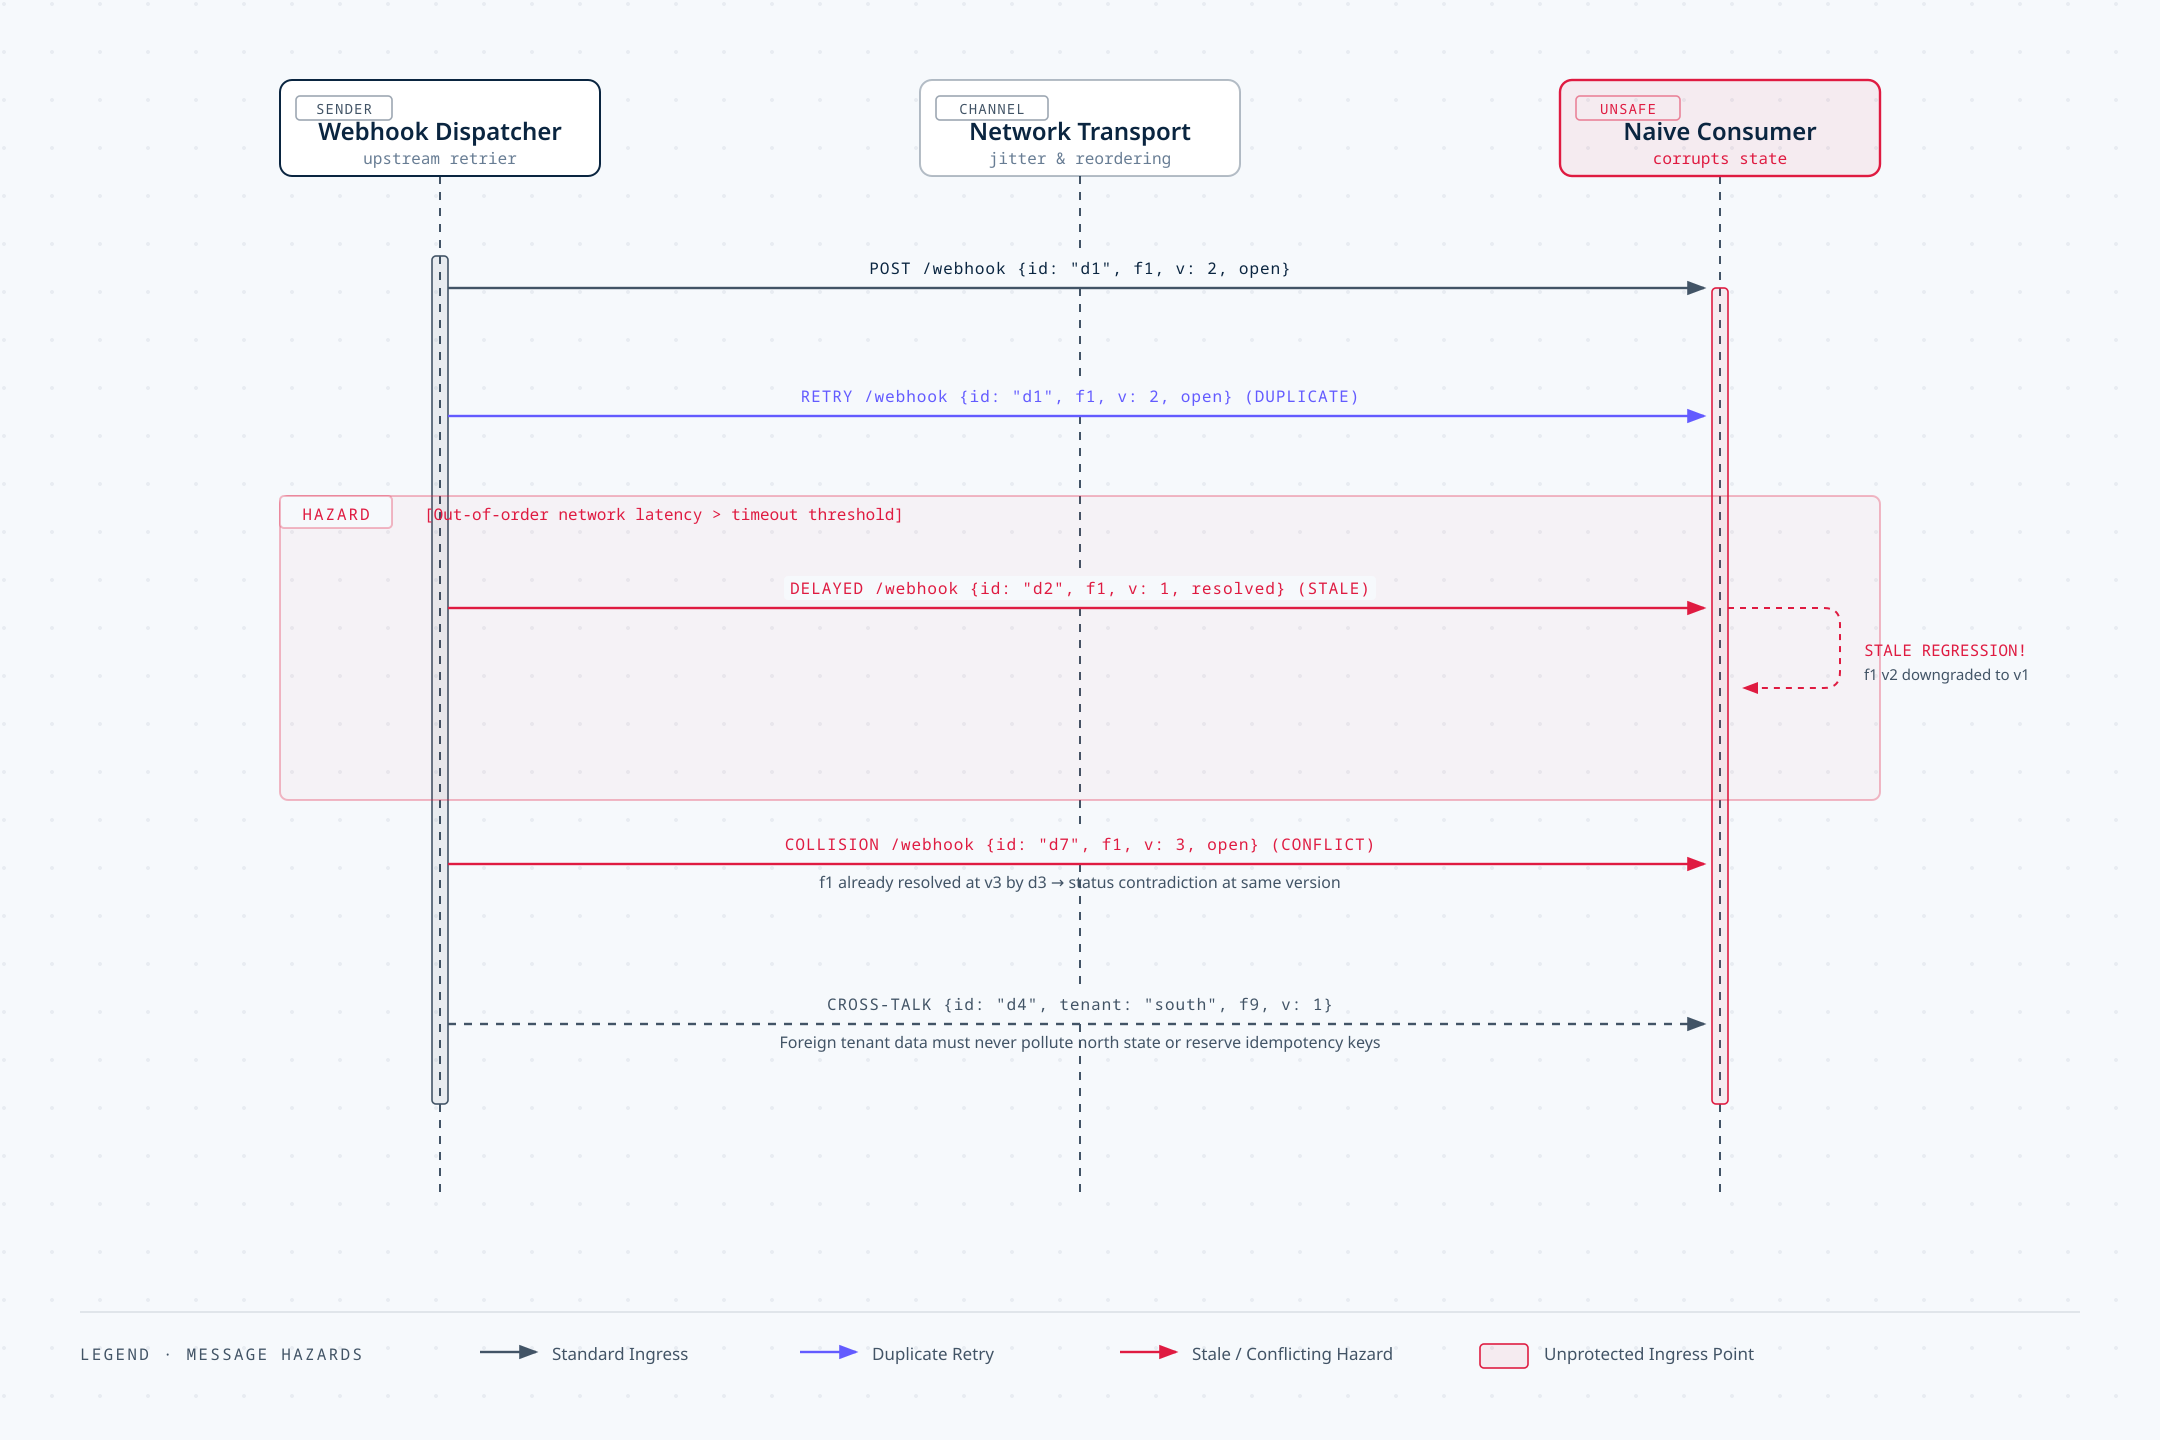
\includegraphics[width=0.90\linewidth]{webhook-redelivery-hazards.png}
\caption{Sequence analysis of webhook redeliveries, latency hazards, and state regressions.}
\label{fig:problem_diagram}
\end{figure}

Our objective is a self-contained CLI that ingests synthetic batches into a local JSON state file while preserving idempotency and monotonic invariants across process runs.

\section{System Invariants and Formal Contract}

State is partitioned into the \textit{Delivery Registry} (transport identity) and the \textit{Finding Registry} (domain state). A normalized delivery row is a tuple:
\begin{equation}
D = \langle \text{id}, \tau, \phi, v, \sigma \rangle, \quad \text{id},\tau,\phi \in \Sigma^+, \; v \in \mathbb{Z}^+, \; \sigma \in \{\text{open}, \text{resolved}\}
\end{equation}

\begin{itemize}[leftmargin=1.5em, noitemsep, topsep=2pt]
    \item \textbf{Invariant 1 (Tenant \& Schema Gate):} Rows failing schema validation or matching $\tau \neq \tau_{\text{CLI}}$ return \texttt{rejected} without reserving an idempotency key or leaking foreign payloads.
    \item \textbf{Invariant 2 (Delivery Identity Gate):} For a known $\text{id}$ with stored payload $P_{\text{stored}} = \langle \tau, \phi, v, \sigma \rangle$:
    \begin{equation}
    \text{Outcome}(\text{id}) = \begin{cases}
    \text{duplicate}, & P_{\text{in}} = P_{\text{stored}} \\
    \text{rejected (delivery conflict)}, & P_{\text{in}} \neq P_{\text{stored}}
    \end{cases}
    \end{equation}
    Neither outcome mutates findings.
    \item \textbf{Invariant 3 (Immediate Key Reservation):} Every valid, unseen $\text{id}$ is recorded in $\text{state}[\texttt{"deliveries"}]$ \textit{before} version comparison, even if its version is stale, redundant, or conflicting.
    \item \textbf{Invariant 4 (Monotonic Progression):} Given finding state $(v_{\text{curr}}, \sigma_{\text{curr}})$:
    \begin{equation}
    \text{Outcome}(v_{\text{in}}, \sigma_{\text{in}}) = \begin{cases}
    \text{applied}, & v_{\text{in}} > v_{\text{curr}} \implies \text{update } (v_{\text{in}}, \sigma_{\text{in}}) \\
    \text{stale}, & v_{\text{in}} < v_{\text{curr}} \implies \text{no-op} \\
    \text{redundant}, & v_{\text{in}} = v_{\text{curr}} \land \sigma_{\text{in}} = \sigma_{\text{curr}} \implies \text{no-op} \\
    \text{rejected}, & v_{\text{in}} = v_{\text{curr}} \land \sigma_{\text{in}} \neq \sigma_{\text{curr}} \implies \text{no-op}
    \end{cases}
    \end{equation}
    \item \textbf{Invariant 5 (Atomic Durability):} State is committed only after a valid batch via a sibling temporary file and POSIX \texttt{os.replace}. Corrupt or foreign state files exit \texttt{2} with zero byte changes.
\end{itemize}

\section{Architecture and Decision Records (ADR)}

Figure~\ref{fig:decision_flow} depicts the two-tier ingestion pipeline, and Table~\ref{tab:adr_matrix} summarizes the six core ADRs.

\begin{figure}[htbp]
\centering
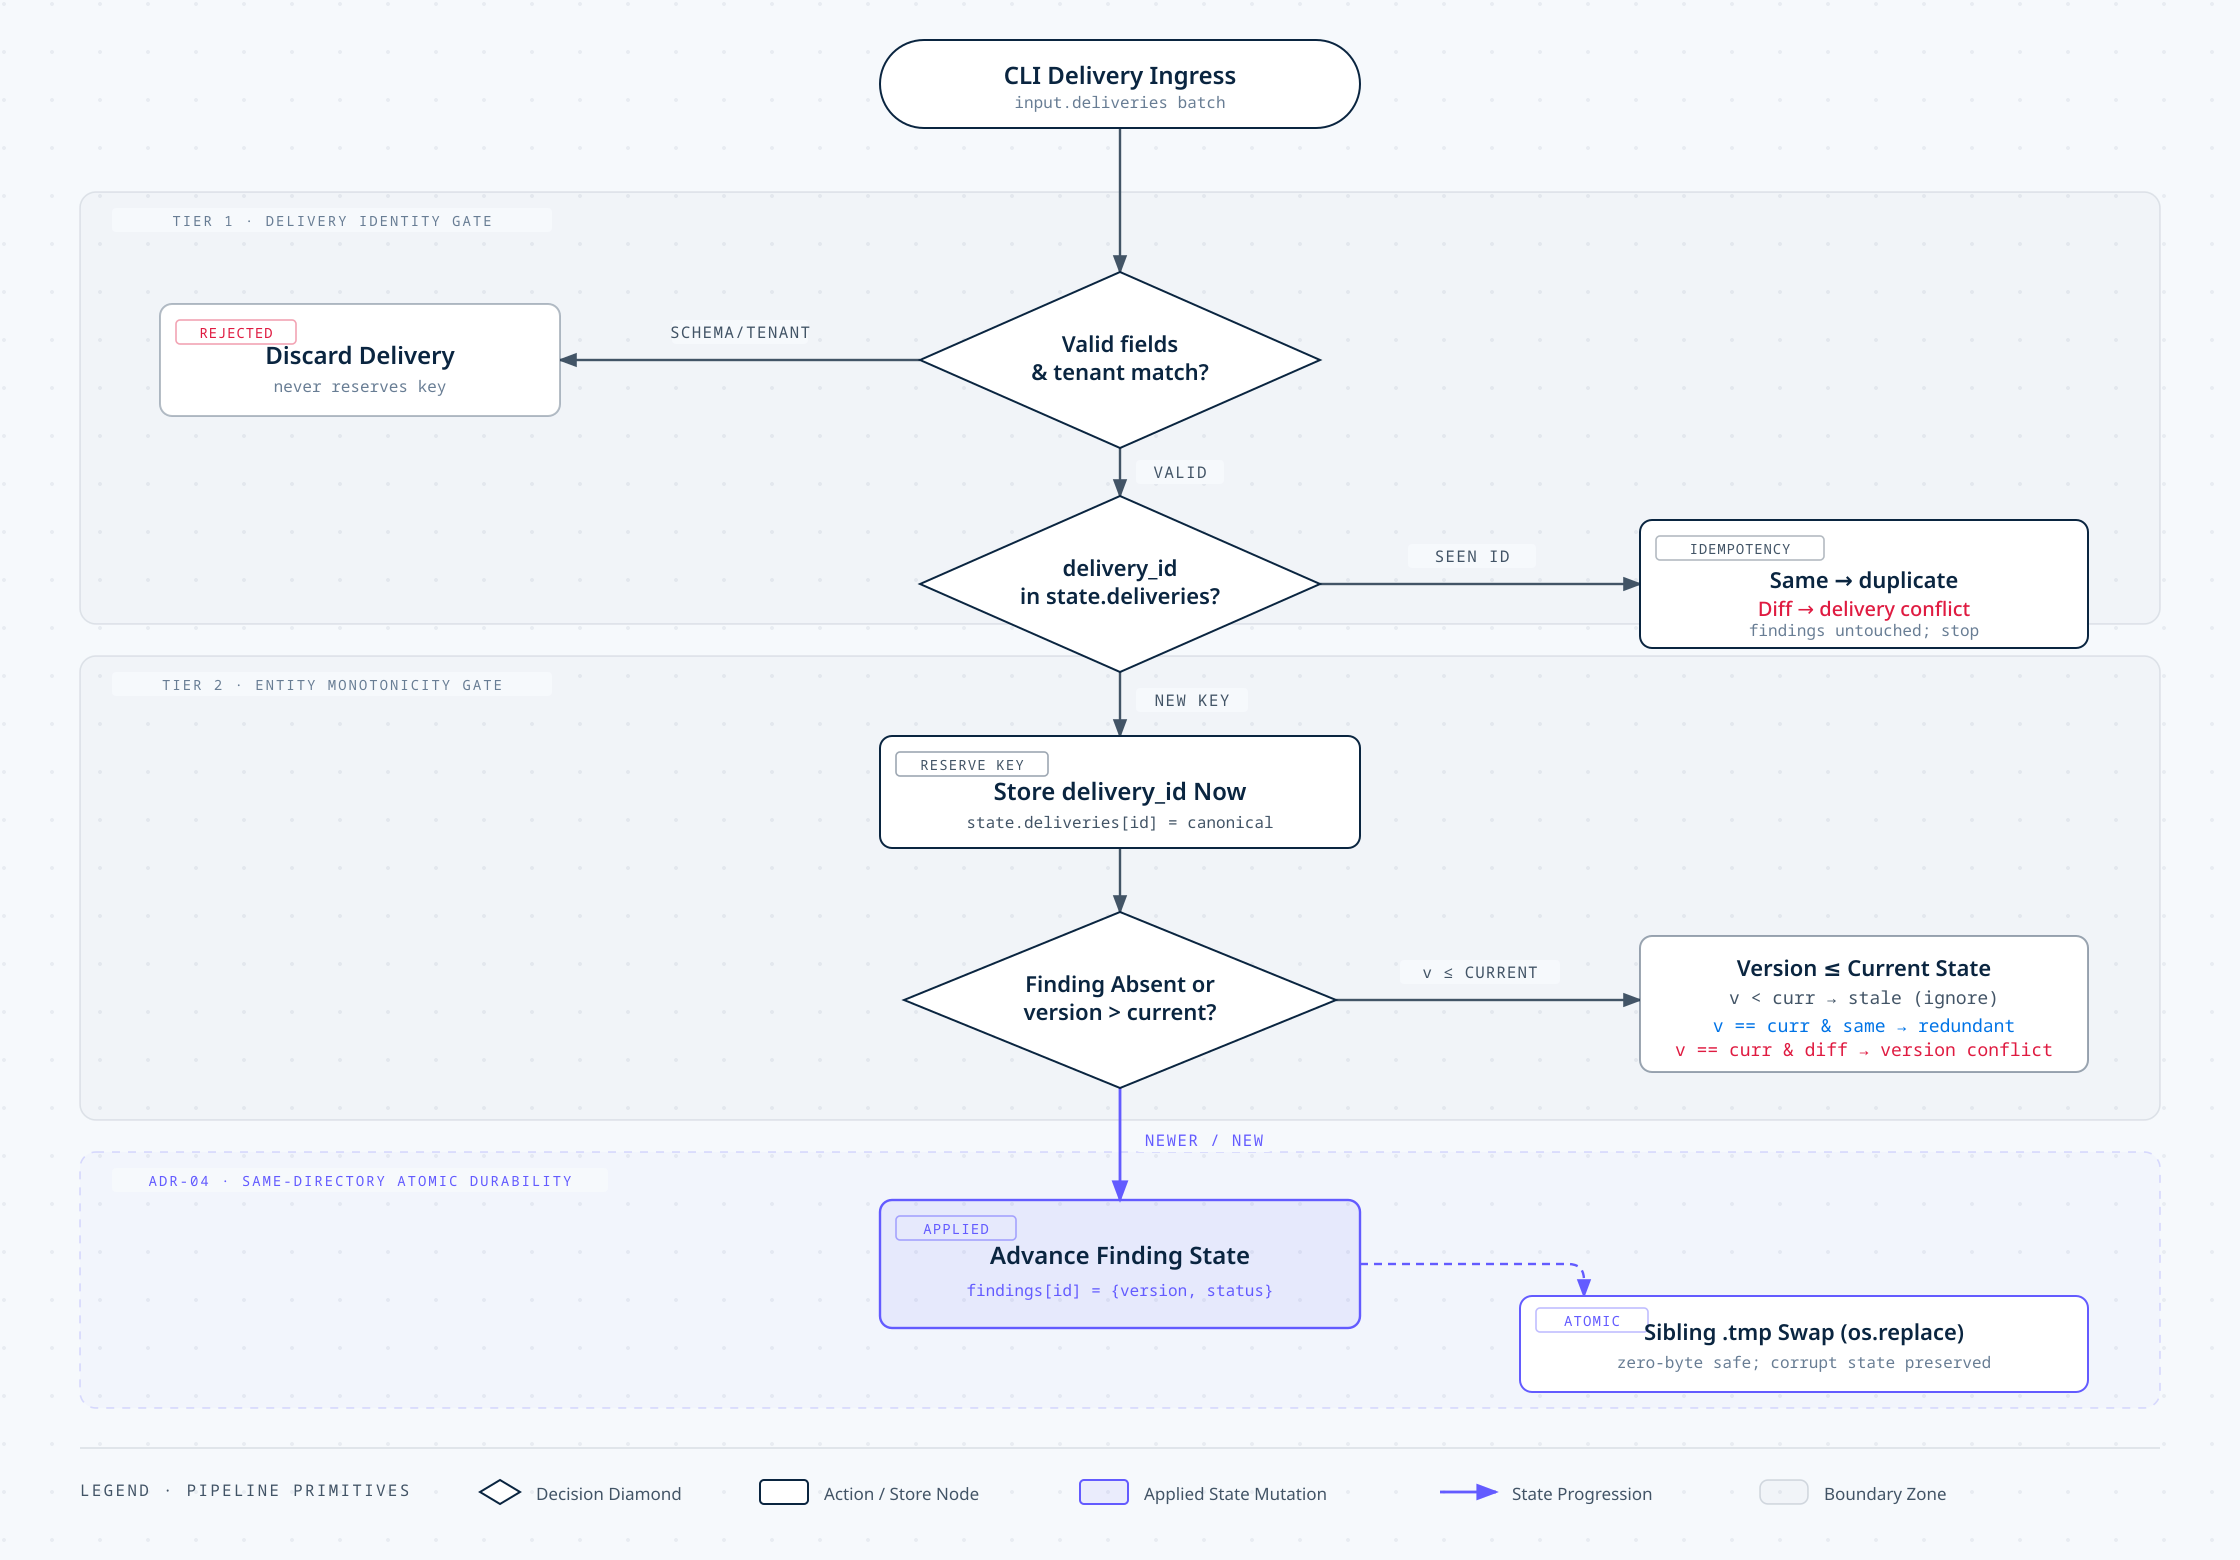
\includegraphics[width=0.92\linewidth]{idempotent-pipeline-architecture.png}
\caption{Two-tier ingestion architecture decoupling transport deduplication from domain monotonicity, backed by sibling-file atomic POSIX persistence (ADR-04).}
\label{fig:decision_flow}
\end{figure}

\begin{table}[htbp]
\centering\footnotesize
\renewcommand{\arraystretch}{1.15}
\caption{Architectural Decision Record (ADR) Summary Matrix}
\label{tab:adr_matrix}
\begin{tabularx}{\textwidth}{@{}llp{3.6cm}p{3.4cm}X@{}}
\toprule
\textbf{ID} & \textbf{Area} & \textbf{Chosen Architecture} & \textbf{Alternative Rejected} & \textbf{Rationale} \\ \midrule
\textbf{ADR-01} & Ingestion & Sequential loop with live mutation & Pre-filtering (\texttt{seen = set()}) & Preserves 1-based row indexing and intra-batch transitions. \\
\textbf{ADR-02} & Pipeline & Two-tier: Delivery Gate $\rightarrow$ Entity Gate & Single unified conditional & Separates transport replay from domain version rules. \\
\textbf{ADR-03} & Key Storage & Reserve valid ID before version check & Lazy reservation on \texttt{applied} & Ensures version conflicts (Row 9) deduplicate on replay. \\
\textbf{ADR-04} & Durability & Sibling temp file + \texttt{os.replace} & In-place \texttt{open(path, "w")} & Prevents 0-byte truncation on crash and cross-mount copies. \\
\textbf{ADR-05} & Integrity & Fail-fast (exit 2) on corrupt state & Silent fallback to empty state & Guarantees forensic byte preservation on invalid state files. \\
\textbf{ADR-06} & Type Safety & \texttt{type(v) is int} (excludes \texttt{bool}) & \texttt{isinstance(v, int)} & Rejects \texttt{"version": true} since \texttt{bool} subclasses \texttt{int}. \\ \bottomrule
\end{tabularx}
\end{table}

\subsection{Row 9 Key Reservation Trap (ADR-03) \& Crash Atomicity (ADR-04)}
\textbf{Row 9 Trap:} In \texttt{primary.json}, Row 9 ($\langle \text{d7}, \text{north}, \text{f1}, 3, \text{open} \rangle$) collides with finding \texttt{f1} at $\{v=3, \text{resolved}\}$ (set by Row 5, \texttt{d3}), yielding \texttt{rejected} (\texttt{version conflict}). Discarding \texttt{d7} causes Run 2 replay to re-evaluate \texttt{d7} as a conflict (\texttt{duplicate: 5, rejected: 4}). Reserving \texttt{d7} immediately after schema validation converts Run 2 into a \texttt{duplicate}, matching the required \texttt{duplicate: 6, rejected: 3}.

\textbf{POSIX Atomicity:} Opening a file with \texttt{"w"} invokes \texttt{truncate(2)} immediately, risking data loss on crash. Staging in \texttt{/tmp} risks cross-filesystem (\texttt{EXDEV}) non-atomic copies. Writing to \texttt{.filename.tmp} in the target parent directory guarantees a single-inode atomic swap via \texttt{os.replace}.

\section{Human-AI Collaborative Verification}

Engagement began with a zero-code conceptual prompt (\texttt{ai\_use/01-Explanation.md}) to establish invariants and test boundaries prior to coding:
\begin{calloutbox}{Developer Prompt (\texttt{ai\_use/01-Explanation.md})}
\footnotesize\textit{"Explain the problem to me clearly before I start solving it. Break down the requirements, explain what is expected from me, provide practical examples and edge cases, and suggest how I should approach the problem step by step. Do not give me the solution, write code, or implement anything."}
\end{calloutbox}

All AI outputs were verified against fixture traces:
\begin{itemize}[leftmargin=1.5em, noitemsep, topsep=2pt]
    \item \textbf{Accepted (ADR-04):} Adopted sibling temporary file staging + \texttt{Path.replace()} with \texttt{unlink()} cleanup.
    \item \textbf{Corrected Hallucination (ADR-03):} AI skipped saving non-applied keys; corrected via Row 9 replay trace to reserve keys immediately upon schema validation.
    \item \textbf{Rejected (ADR-01):} Rejected batch pre-deduplication (\texttt{seen = set()}) because it breaks 1-based indexing and hides delivery conflicts.
    \item \textbf{Corrected Type Check (ADR-06):} Replaced AI's \texttt{isinstance(v, int)} with \texttt{type(v) is int} to block \texttt{bool} coercion.
\end{itemize}

\section{Core Implementation Artifacts}

Listings~\ref{lst:validation}--\ref{lst:ingest} present the production implementation in \texttt{app.py}.

\begin{lstlisting}[language=Python,caption={Row validation with strict boolean exclusion (\texttt{app.py}).},label={lst:validation}]
def validate_delivery_row(
    row: typing.Any, expected_tenant: str
) -> tuple[bool, dict[str, typing.Any] | None, str, str | None]:
    if not isinstance(row, dict):
        return False, None, "", "row must be an object"

    raw_delivery_id = row.get("delivery_id")
    raw_tenant = row.get("tenant")
    raw_finding_id = row.get("finding_id")
    version = row.get("version")
    raw_status = row.get("status")

    delivery_id = str(raw_delivery_id).strip() if isinstance(raw_delivery_id, str) else ""

    if not isinstance(raw_delivery_id, str) or not raw_delivery_id.strip():
        return False, None, delivery_id, "delivery_id must be a non-empty string"
    if not isinstance(raw_tenant, str) or not raw_tenant.strip():
        return False, None, delivery_id, "tenant must be a non-empty string"
    if not isinstance(raw_finding_id, str) or not raw_finding_id.strip():
        return False, None, delivery_id, "finding_id must be a non-empty string"

    tenant = raw_tenant.strip()
    if tenant != expected_tenant:
        return False, None, delivery_id, f"foreign tenant: {tenant}"

    # Strict type identity check excluding bool
    if type(version) is not int or isinstance(version, bool) or version <= 0:
        return False, None, delivery_id, "version must be a positive integer"

    if not isinstance(raw_status, str):
        return False, None, delivery_id, "status must be a string"
    status = raw_status.strip()
    if status not in VALID_STATUSES:
        return False, None, delivery_id, f"status must be 'open' or 'resolved', got '{status}'"

    canonical = {
        "tenant": tenant,
        "finding_id": raw_finding_id.strip(),
        "version": version,
        "status": status,
    }
    return True, canonical, delivery_id, None
\end{lstlisting}

\begin{lstlisting}[language=Python,caption={Crash-safe sibling temporary file serialization (\texttt{app.py}).},label={lst:atomic_save}]
def save_state(state: dict[str, typing.Any], state_path: pathlib.Path) -> None:
    """Atomically save state JSON file via a temporary file in the same directory."""
    target = state_path.resolve()
    target.parent.mkdir(parents=True, exist_ok=True)
    temp_path = target.with_name(f".{target.name}.tmp")
    try:
        content = json.dumps(state, indent=2, sort_keys=True) + "\n"
        temp_path.write_text(content, encoding="utf-8")
        temp_path.replace(target)
    except Exception as error:
        if temp_path.exists():
            try:
                temp_path.unlink()
            except OSError:
                pass
        raise ValueError(f"failed to save state: {error}") from error
\end{lstlisting}

\begin{lstlisting}[language=Python,caption={Two-tier sequential ingestion loop (\texttt{app.py}).},label={lst:ingest}]
for row_idx, row in enumerate(deliveries, start=1):
    is_valid, canonical, delivery_id, reason = validate_delivery_row(row, arguments.tenant)
    if not is_valid:
        results.append({"row": row_idx, "delivery_id": delivery_id, "outcome": "rejected", "reason": reason})
        counts["rejected"] += 1
        continue

    # Tier 1: Delivery Identity Gate
    if delivery_id in state["deliveries"]:
        stored = state["deliveries"][delivery_id]
        if stored == canonical:
            outcome, reason = "duplicate", "duplicate delivery"
            counts["duplicate"] += 1
        else:
            outcome, reason = "rejected", "delivery conflict"
            counts["rejected"] += 1
        results.append({"row": row_idx, "delivery_id": delivery_id, "outcome": outcome, "reason": reason})
        continue

    # Step 3: Immediate Key Reservation
    state["deliveries"][delivery_id] = canonical

    # Tier 2: Entity Monotonicity Gate
    finding_id = canonical["finding_id"]
    version, status = canonical["version"], canonical["status"]
    current = state["findings"].get(finding_id)

    if current is None or version > current["version"]:
        state["findings"][finding_id] = {"version": version, "status": status}
        outcome, reason = "applied", "finding updated"
        counts["applied"] += 1
    elif version < current["version"]:
        outcome, reason = "stale", "stale version"
        counts["stale"] += 1
    else:  # version == current["version"]
        if status == current["status"]:
            outcome, reason = "redundant", "redundant status"
            counts["redundant"] += 1
        else:
            outcome, reason = "rejected", "version conflict"
            counts["rejected"] += 1

    results.append({"row": row_idx, "delivery_id": delivery_id, "outcome": outcome, "reason": reason})
\end{lstlisting}

\section{Empirical Verification and Edge Case Trace}

\textbf{Acceptance Runs:}
\begin{enumerate}[leftmargin=1.5em, noitemsep, topsep=2pt]
    \item \textbf{Run 1 (Fresh Primary):} \texttt{applied: 3, duplicate: 1, stale: 1, redundant: 0, rejected: 4} (Exit \texttt{0}).
    \item \textbf{Run 2 (Primary Replay):} \texttt{applied: 0, duplicate: 6, stale: 0, redundant: 0, rejected: 3} (Exit \texttt{0}; rows 1, 2, 4, 5, 8, 9 deduplicate).
    \item \textbf{Run 3 (Secondary):} \texttt{applied: 2, duplicate: 0, stale: 0, redundant: 1, rejected: 0} (Exit \texttt{0}; \texttt{f1}: $\{v=4, \text{open}\}$, \texttt{f2}: $\{v=2, \text{resolved}\}$).
\end{enumerate}

\begin{table}[htbp]
\centering\footnotesize
\renewcommand{\arraystretch}{1.1}
\caption{Automated 18-Test Regression Suite (\texttt{tests/app\_test.py})}
\label{tab:test_results}
\begin{tabularx}{\textwidth}{@{}lXl|lXl@{}}
\toprule
\textbf{Test Name} & \textbf{Verified Invariant} & \textbf{St.} & \textbf{Test Name} & \textbf{Verified Invariant} & \textbf{St.} \\ \midrule
\texttt{whenHelpRequested} & Usage stdout, exit 0 & \textcolor{ggreen}{\textbf{P}} & \texttt{whenVersionZero} & $v \le 0$ rejected & \textcolor{ggreen}{\textbf{P}} \\
\texttt{whenInputMissing} & Stderr diagnostic, exit 2 & \textcolor{ggreen}{\textbf{P}} & \texttt{whenVersionBoolean} & Bool exclusion guard & \textcolor{ggreen}{\textbf{P}} \\
\texttt{whenJsonMalformed} & Corrupt JSON, exit 2 & \textcolor{ggreen}{\textbf{P}} & \texttt{whenMissingField} & Missing key rejected & \textcolor{ggreen}{\textbf{P}} \\
\texttt{whenPrimaryRun} & Fresh counts (3/1/1/0/4) & \textcolor{ggreen}{\textbf{P}} & \texttt{whenMismatch} & Tenant mismatch, exit 2 & \textcolor{ggreen}{\textbf{P}} \\
\texttt{whenPrimaryReplayed} & Replay counts (0/6/0/0/3) & \textcolor{ggreen}{\textbf{P}} & \texttt{whenStatusCase} & \texttt{"OPEN"} rejected & \textcolor{ggreen}{\textbf{P}} \\
\texttt{whenSecondaryRun} & Counts (2/0/0/1/0) & \textcolor{ggreen}{\textbf{P}} & \texttt{whenDeliveryIdInt} & Non-str ID rejected & \textcolor{ggreen}{\textbf{P}} \\
\texttt{whenStateMalformed} & 0-byte mutation, exit 2 & \textcolor{ggreen}{\textbf{P}} & \texttt{whenEmptyDeliveries} & Empty batch succeeds & \textcolor{ggreen}{\textbf{P}} \\
\texttt{whenWhitespace} & Trims canonical strings & \textcolor{ggreen}{\textbf{P}} & \texttt{whenStateTenantMismatch} & Foreign state preserved & \textcolor{ggreen}{\textbf{P}} \\
\texttt{whenForeignTenant} & No key reserved & \textcolor{ggreen}{\textbf{P}} & \texttt{whenVersionConflict} & Row 9 replay proof & \textcolor{ggreen}{\textbf{P}} \\ \bottomrule
\end{tabularx}
\end{table}

\begin{table}[htbp]
\centering\footnotesize
\renewcommand{\arraystretch}{1.12}
\caption{Row-by-Row Execution Trace of \texttt{inputs/primary.json}}
\label{tab:row_trace}
\begin{tabularx}{\textwidth}{@{}cclXlcc@{}}
\toprule
\textbf{Row} & \textbf{ID} & \textbf{Payload} & \textbf{Evaluation Step} & \textbf{Run 1} & \textbf{Key Stored?} & \textbf{State Mutation} \\ \midrule
1 & \texttt{d1} & \texttt{f1}, $v=2$, \texttt{open} & Finding absent $\implies$ init & \texttt{applied} & \textbf{Yes} & \texttt{f1}: $\{v=2, \text{open}\}$ \\
2 & \texttt{d1} & \texttt{f1}, $v=2$, \texttt{open} & Seen \texttt{d1} $\land$ identical payload & \texttt{duplicate} & Stored & None \\
3 & \texttt{d1} & \texttt{f1}, $v=2$, \texttt{resolved} & Seen \texttt{d1} $\land$ conflicting status & \texttt{rejected} & Stored & None \\
4 & \texttt{d2} & \texttt{f1}, $v=1$, \texttt{resolved} & New ID; $v=1 < 2$ (stale) & \texttt{stale} & \textbf{Yes} & None \\
5 & \texttt{d3} & \texttt{f1}, $v=3$, \texttt{resolved} & New ID; $v=3 > 2$ (advance) & \texttt{applied} & \textbf{Yes} & \texttt{f1}: $\{v=3, \text{resolved}\}$ \\
6 & \texttt{d4} & \texttt{f9}, $v=1$, \texttt{open} (south) & Foreign tenant validation fail & \texttt{rejected} & \textbf{No} & None \\
7 & \texttt{d5} & \texttt{f2}, $v=0$, \texttt{open} & Version $0 \le 0$ validation fail & \texttt{rejected} & \textbf{No} & None \\
8 & \texttt{d6} & \texttt{f2}, $v=1$, \texttt{open} & Finding absent $\implies$ init & \texttt{applied} & \textbf{Yes} & \texttt{f2}: $\{v=1, \text{open}\}$ \\
9 & \texttt{d7} & \texttt{f1}, $v=3$, \texttt{open} & New ID; $v=3 \land \text{open} \neq \text{resolved}$ & \texttt{rejected} & \textbf{Yes} & None \\ \bottomrule
\end{tabularx}
\end{table}

\section{Scope Boundaries and Conclusion}

\textbf{Scope \& Next Steps:} Process-level file locks (\texttt{fcntl.flock}) and SQLite backends were intentionally deferred per the sequential JSON CLI specification. For high-throughput production streams, future iterations will introduce streaming JSON parsers (\texttt{ijson}) and SQLite WAL-mode storage.

\textbf{Conclusion:} Decoupling delivery deduplication from entity monotonicity—backed by immediate key reservation and POSIX sibling-file replacement—guarantees deterministic state consistency across process lifecycles.

\section*{Appendix: Persisted State After Run 3}

\begin{lstlisting}[language=Python,caption={Final serialized state (\texttt{scratch-state.json}) after Run 3.},label={lst:state_json}]
{
  "deliveries": {
    "d1": {"finding_id": "f1", "status": "open", "tenant": "north", "version": 2},
    "d2": {"finding_id": "f1", "status": "resolved", "tenant": "north", "version": 1},
    "d3": {"finding_id": "f1", "status": "resolved", "tenant": "north", "version": 3},
    "d6": {"finding_id": "f2", "status": "open", "tenant": "north", "version": 1},
    "d7": {"finding_id": "f1", "status": "open", "tenant": "north", "version": 3},
    "s1": {"finding_id": "f1", "status": "open", "tenant": "north", "version": 4},
    "s2": {"finding_id": "f2", "status": "open", "tenant": "north", "version": 1},
    "s3": {"finding_id": "f2", "status": "resolved", "tenant": "north", "version": 2}
  },
  "findings": {
    "f1": {"status": "open", "version": 4},
    "f2": {"status": "resolved", "version": 2}
  },
  "tenant": "north"
}
\end{lstlisting}

\end{document}